\documentclass[
	classe=$1^{ere}STI2D$,
	headerTitle=Activité,
	twocolumn,
	landscape
]{exercice}

\usepackage{tkz-tab}
\usetikzlibrary{calc}

\setlength{\leftmarginii}{0.2cm}
\setlength{\columnsep}{0.9cm}

\renewcommand{\correction}[1]{\correctionOr{\textcolor{red}{#1}}{}}

\title{Activité : Optimiser ses recettes}

\begin{document}

\newcommand{\Enonce}{
	\maketitle

	Une entreprise artisanale fabrique des chaises de salon. Elle peut en fabriquer maximum $25$ par jour. \medskip

	Le coût total de fabrication de $n$ chaises est définit par la fonction

	$C(n) = -n² + 58n + 120$ (en euros). \medskip

	Ces chaises sont ensuite toutes vendues : vendre $n$ chaises rapporte à l'entreprise $R(n) = -2n² + 85n$ de recettes (en euros).

	\begin{enumerate}
		\item Calculer la formule donnant le bénéfice $B(n)$ réalisé par l'entreprise en vendant $n$ chaises. \correction{$B(n) = -n² + 29n - 120$}
		\item Calculer $B(1)$. L'entreprise gagne-t-elle de l'argent en vendant une seule chaise ? \correction{$B(1) = -1 + 29 - 120 = -84€$}
		\item Montrer que $B(n)$ peut s'écrire $-(n - 5)(n - 24)$. \correction{Double distributivité}
		\item Remplir les trois premières lignes du tableau de signes ci-dessous.
		      \begin{center}
			      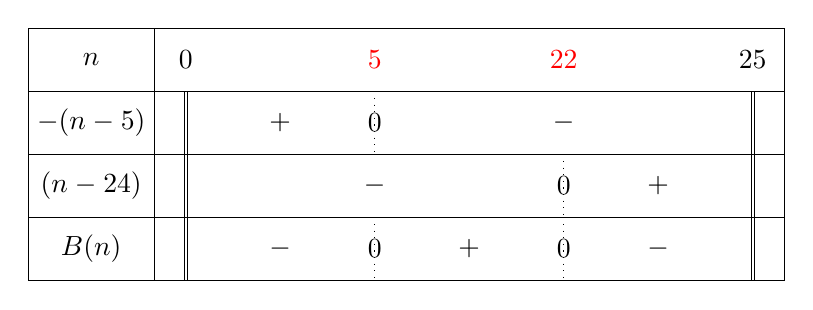
\begin{tikzpicture}[scale=0.8]
				      \tkzTabInit{$n$ / 1, $-(n - 5)$ / 1, $(n - 24)$ / 1, $B(n)$ / 1}{$0$, \correction{$5$}, \correction{$22$}, $25$}
				      \correctionOr{\tkzTabLine{d, +, z, , -, , d}}{}
				      \correctionOr{\tkzTabLine{d, , -, , z, +, d}}{}
				      \correctionOr{\tkzTabLine{d, -, z, +, z, -, d}}{}
			      \end{tikzpicture}
		      \end{center}

		\item On sait que $B(n) = -(n - 5)(n - 24)$.

		      Ainsi,
		      \begin{itemize}
			      \item Si $-(n - 5)$ est positif et $(n - 24)$ est négatif, $B(n)$ est \correctionOr{\textcolor{red}{négatif}}{................}.
			      \item Si $-(n - 5)$ est négatif et $(n - 24)$ est négatif, $B(n)$ est \correctionOr{\textcolor{red}{positif}}{...............}.
			      \item Si $-(n - 5)$ est négatif et $(n - 24)$ est positif, $B(n)$ est \correctionOr{\textcolor{red}{négatif}}{................}.
		      \end{itemize}

		      Remplir alors la dernière ligne du tableau de signes.
		\item Avec la calculatrice, donner un encadrement du bénéfice maximal de l'entreprise. \medskip

		      Dans la numworks, on peut :

		      \begin{itemize}
			      \item Aller dans l'application « fonctions », et entrer l'expression de la fonction $B$.
			      \item Aller sur « Afficher les valeurs ».
			      \item Aller sur « Régler l'intervalle » pour avoir toutes les valeurs entre $0$ et $25$.
		      \end{itemize}

		      \ifdefined\makeCorrection
			      \newcommand{\cellWidth}{1.2}
			      \begin{center}
				      \begin{tikzpicture}
					      \draw (0,0) -- ++(14*\cellWidth,0);
					      \draw (0,-1) -- ++(14*\cellWidth,0);
					      \draw (0,-2) -- ++(14*\cellWidth,0);
					      \draw (\cellWidth,-3) -- ++(13*\cellWidth,0);
					      \draw (\cellWidth,-4) -- ++(13*\cellWidth,0);
					      \draw (0,0) -- (0,-2);
					      \draw (1*\cellWidth,0) -- ++(0,-4);
					      \node at (0.5*\cellWidth,-0.5) {$n$};
					      \node at (0.5*\cellWidth,-1.5) {$B(n)$};

					      \foreach \n in {0,...,12} {
							      \pgfmathsetmacro\ColumnPos{\cellWidth*(1.5+\n)}
							      \draw (\cellWidth*0.5+\ColumnPos,0) -- ++(0,-2);
							      \node at (\ColumnPos,-0.5) {$\n$};
							      \pgfmathsetmacro\Bn{-(\n - 5)*(\n - 24)}
							      \node at (\ColumnPos,-1.5) {$\Bn$};
						      }
					      \foreach \n in {13,...,25} {
							      \pgfmathsetmacro\ColumnPos{\cellWidth*(\n-11.5)}
							      \draw (\cellWidth*0.5+\ColumnPos,-2) -- ++(0,-2);
							      \node at (\ColumnPos,-2.5) {$\n$};
							      \pgfmathsetmacro\Bn{-(\n - 5)*(\n - 24)}
							      \node at (\ColumnPos,-3.5) {$\Bn$};
						      }
				      \end{tikzpicture}
			      \end{center}
		      \fi
	\end{enumerate}
}

\Enonce

\ifdefined\makeCorrection
\else
	\newpage
	\Enonce
\fi

\end{document}